\chapter{Functionality}
\label{chapter:functionality}

The goal of the project ACE is to create a plattform independent collaborative text editor. To achieve that goal the editor must satisfy basic text editor functionality as well as collaborative editor functionality.\\

\begin{figure}[H]
\begin{center}
  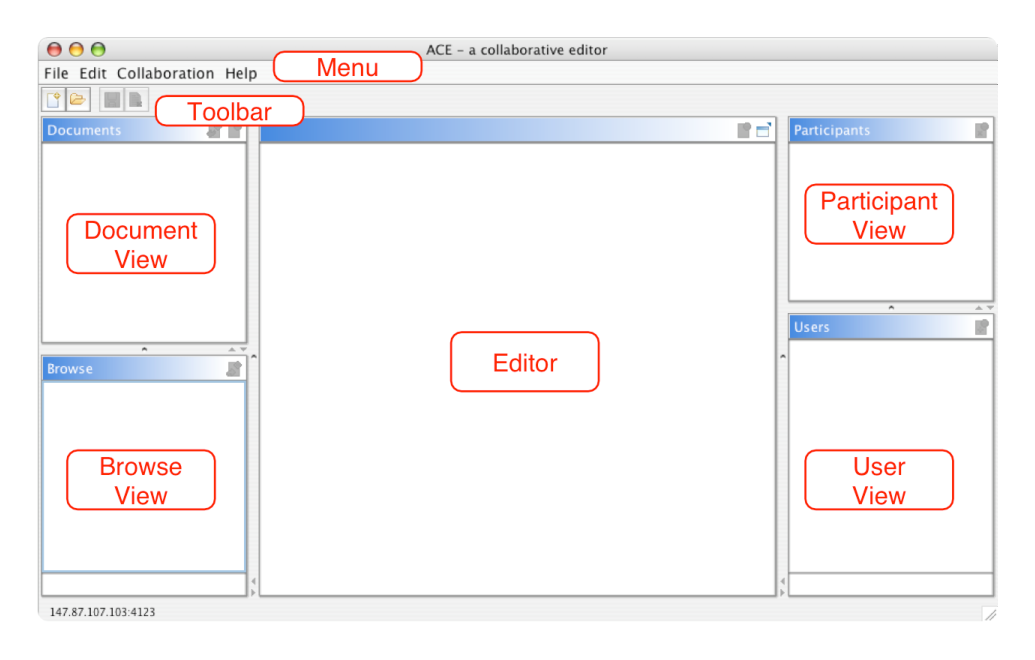
\includegraphics[height=3.1in, width=5.1in]{../images/finalreport/application_ace_overview.eps}
\caption{ACE Overview}
\end{center}
\end{figure}

A basic text editor must have features like create new, load and save documents. Further it would be userfriendly to have multiple documents open at the same time and switch between them. Operations like cut/copy/paste and undo/redo shouldnt be missing. A more detailed description of the goals can be found in the \textit{System Requirement: 2.1 Mandatory Goals}. See section \ref{sect:algorithm.undoredo} for a description about the lack of undo/redo in our editor.\\

Besides the basic text editor functions, a collaborative text editor must support the \textit{publication} of documents. The published documents should be discovered automatically by all other users running a collaborative text editor in the same local area network (LAN). This leads to the situation that every user has a list of documents that have been published by other users in the same network. A user can \textit{join} the editing session for such a published document. This means that he start participating the collaborative editing of the document and he is able to insert, remove or update the content of the document. He also can be \textit{invited} by the owner (publisher) of the published document. To counteract misbehaviour the publisher can \textit{kick} invited users which results in a blacklist entry until they receive a re-invite.

The editor should look very simple and the components should be clearly arranged for the user friendlyness. To improve the intuitive handling of the editor buttons with meaningful images should be positioned at the right and logical place. Different colors that are used to highlight the written text and to draw the cursor positions (or selections) making the participants well distinguishable. \\

\begin{figure}[H]
\begin{center}
  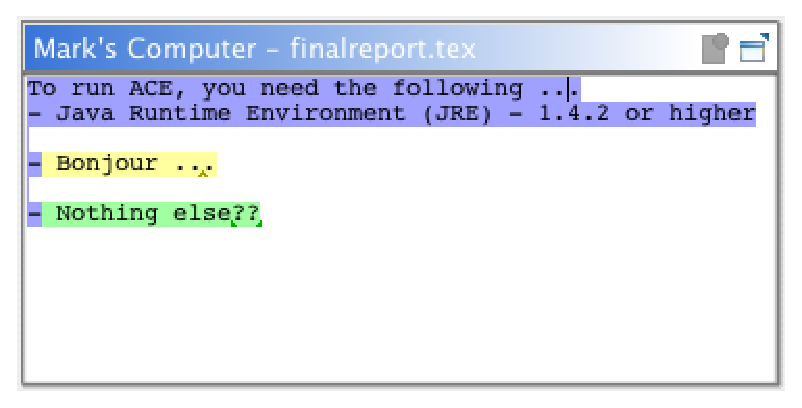
\includegraphics[height=2.5in, width=5.12in]{../images/usermanual/editor_collab_3users.eps}
\caption{Three Users writing in one Document}
\end{center}
\end{figure}

Based on these facts we defined mandatory, optional and non-goals for our diploma work in \textit{System Requirements: Project Goals}. A description of the preview work can be found in \ref{sect:overview.previouswork}.
